\documentclass[kdmile,a4paper]{kdmile}

\usepackage[utf8]{inputenc}
\usepackage[T1]{fontenc}
\usepackage[brazilian]{babel}
\usepackage{amsmath}
\usepackage{amssymb}
\usepackage{booktabs}
\usepackage{array}
\usepackage{graphicx,url}
\graphicspath{{figures/}}

\newtheorem{theorem}{Theorem}[section]
\newtheorem{conjecture}[theorem]{Conjecture}
\newtheorem{corollary}[theorem]{Corollary}
\newtheorem{proposition}[theorem]{Proposition}
\newtheorem{lemma}[theorem]{Lemma}
\newdef{definition}[theorem]{Definition}
\newdef{remark}[theorem]{Remark}

\markboth{Araújo Júnior and Caminha Neto}
{Garbage Bag Detection and Localization}
\title{Garbage Bag Detection and Localization: Comparing YOLOv11m and Gemma 4 31B-QAT}

\author{Jaime Teixeira de Araújo Júnior$^{1}$, Carlos de Oliveira Caminha Neto$^{1}$}

\institute{$^{1}$ Universidade Federal do Ceará (UFC)\\
Fortaleza, CE, Brasil\\
\texttt{jaimejrs@alu.ufc.br, caminha@ufc.br}}


\begin{abstract}
Monitoring garbage bags on public roads requires large-scale inspection under limited operational resources. This study compares YOLOv11m, fine-tuned as a specialized detector, and Gemma 4 31B-QAT, used as a zero-shot vision-language model, for identifying the presence and location of garbage bags in Brazilian street images. YOLOv11m was trained with 5,248 images from two Roboflow garbage-bag datasets and negative sidewalk scenes. Both models were evaluated on a balanced external test set of 560 Google Street View screenshots from multiple Brazilian states, annotated and cross-reviewed by two researchers. Gemma achieved higher F1-score for binary identification (0.9838 versus 0.7600) and higher per-image localization success at intersection over union (IoU) 0.5 (0.3893 versus 0.2714), although both models had low box-level F1-scores. YOLOv11m processed 106.5 images per second, whereas Gemma's average latency was 141.9 times higher. These results reveal an accuracy--latency--localization trade-off and motivate hybrid systems combining fast detection, multimodal confirmation, and human review.
\end{abstract}

\begin{CCSXML}
<ccs2012>
<concept>
<concept_id>10010147.10010257.10010258.10010259</concept_id>
<concept_desc>Computing methodologies~Object detection</concept_desc>
<concept_significance>500</concept_significance>
</concept>
<concept>
<concept_id>10010147.10010257.10010282</concept_id>
<concept_desc>Computing methodologies~Computer vision</concept_desc>
<concept_significance>500</concept_significance>
</concept>
<concept>
<concept_id>10010405.10010469.10010474</concept_id>
<concept_desc>Applied computing~Environmental sciences</concept_desc>
<concept_significance>300</concept_significance>
</concept>
</ccs2012>
\end{CCSXML}
\ccsdesc[500]{Computing methodologies~Object detection}
\ccsdesc[500]{Computing methodologies~Computer vision}
\ccsdesc[300]{Applied computing~Environmental sciences}

\keywords{garbage bag detection, object detection, public administration, vision-language models, YOLOv11m}

\begin{document}

\begin{bottomstuff}
\end{bottomstuff}

\maketitle

\section{Introdução}
\label{sec:introducao}

A gestão de resíduos sólidos urbanos envolve impactos ambientais, sanitários, financeiros e operacionais. No Brasil, a Política Nacional de Resíduos Sólidos atribui aos municípios papel central na organização da coleta e destinação dos resíduos \cite{Brasil2010}, cujos custos dependem diretamente da estrutura operacional adotada \cite{Rodrigues2016}.

A produção de informações territorializadas sobre o descarte irregular de sacos de lixo pode apoiar a priorização de áreas, o planejamento de rotas e a fiscalização. Entretanto, a inspeção manual de grandes volumes de imagens demanda tempo e recursos humanos. Técnicas de visão computacional oferecem a possibilidade de transformar registros visuais de ruas em alertas administrativos, mas sua utilidade depende não apenas da acurácia, como também da velocidade, da ocorrência de falsos alarmes, da rastreabilidade e da infraestrutura necessária para operação.

Detectores da família YOLO localizam rapidamente instâncias e retornam caixas que facilitam a auditoria \cite{Redmon2016YOLO,Ultralytics2024YOLO11}. Modelos de visão e linguagem (VLMs) associam imagens e instruções e podem operar em regime \emph{zero-shot}, sem ajuste no conjunto-alvo \cite{Radford2021CLIP}. Essa flexibilidade reduz o treinamento inicial, mas pode elevar o custo de inferência.

Estudos anteriores mostraram que a análise automatizada de resíduos enfrenta dificuldades associadas a materiais deformáveis, sobrepostos, parcialmente oclusos e inseridos em cenas visualmente carregadas \cite{Bashkirova2022ZeroWaste,Abid2025WasteDetection}. Paralelamente, a supervisão conjunta de imagens e linguagem possibilitou classificação visual \emph{zero-shot} \cite{Radford2021CLIP} e métodos de detecção aberta que combinam conhecimento semântico e localização \cite{Kuo2023FVLM,Jin2024FineGrainedDescriptors}. Comparações entre detectores supervisionados e VLMs fundacionais devem considerar a assimetria do pré-treinamento e o alinhamento dos conceitos aprendidos ao domínio-alvo \cite{Madan2024FewShotVLM}. Apesar desses avanços, a literatura revisada oferece evidência limitada sobre a comparação direta, nas mesmas imagens brasileiras de vias públicas, entre um detector especializado e um grande modelo visão-linguagem para identificar a presença e determinar a localização de sacos de lixo, considerando também o custo de inferência.

Este trabalho investiga as seguintes perguntas de pesquisa:
\begin{itemize}
    \setlength{\itemsep}{0pt}
    \setlength{\parsep}{0pt}
    \setlength{\topsep}{2pt}
    \item \textbf{RQ1:} Como se comparam um detector especializado com \emph{fine-tuning} e um VLM generalista em \emph{zero-shot} na identificação da presença e na localização de sacos de lixo em imagens reais de vias públicas brasileiras?
    \item \textbf{RQ2:} Qual é o trade-off entre desempenho na identificação e localização de sacos de lixo, eficiência computacional e adequação aos diferentes cenários de monitoramento urbano?
\end{itemize}

As principais contribuições são: uma comparação controlada, em imagens brasileiras de vias públicas, entre um detector especializado e um VLM generativo, considerando a identificação da presença de sacos de lixo, sua localização espacial e a eficiência computacional; a análise pareada da identificação binária e da localização dos sacos por caixas delimitadoras; e a caracterização dos cenários em que cada paradigma apresenta maior viabilidade operacional.

\section{Trabalhos Relacionados}
\label{sec:trabalhos-relacionados}

\subsection{Detecção automatizada de sacos de lixo}
\label{sec:deteccao-residuos}

A detecção de objetos busca identificar e localizar instâncias por meio de caixas delimitadoras. Detectores de uma etapa, como o YOLO, realizam a predição conjunta de classes e regiões, favorecendo aplicações de baixa latência \cite{Redmon2016YOLO,Ultralytics2024YOLO11}. No domínio de resíduos, o conjunto ZeroWaste evidenciou dificuldades provocadas por materiais deformáveis, sobreposição, oclusão e fundos visualmente carregados \cite{Bashkirova2022ZeroWaste}. Avaliações recentes também demonstraram que deslocamento de domínio e formulação linguística afetam o desempenho de métodos supervisionados e de vocabulário aberto \cite{Abid2025WasteDetection}. Embora esses trabalhos cubram resíduos heterogêneos, este estudo adota um recorte mais estrito: apenas sacos usados para acondicionar lixo constituem o objeto-alvo, excluindo resíduos avulsos.

\subsection{Modelos de visão e linguagem}
\label{sec:modelos-visao-linguagem}

VLMs aprendem representações conjuntas de imagens e textos. O CLIP demonstrou a transferência desse conhecimento para classificação \emph{zero-shot} \cite{Radford2021CLIP}; o paradigma foi combinado a componentes de detecção em abordagens de vocabulário aberto \cite{Kuo2023FVLM}. Descrições detalhadas podem melhorar o alinhamento entre conceitos e regiões \cite{Jin2024FineGrainedDescriptors}, enquanto VLMs generativos tratam tarefas visuais por instruções e saídas estruturadas \cite{Wang2023VisionLLM}.

Reconhecimento global e localização fina não são problemas equivalentes; métodos híbridos combinam VLMs com componentes especializados para reduzir essa diferença \cite{Lin2024VLSAM}. Aqui, o Gemma é avaliado como modelo generativo \emph{zero-shot}, produzindo decisões binárias e coordenadas por instruções, enquanto o YOLOv11m representa um detector ajustado ao domínio de treinamento.

O modelo multimodal foi carregado pelo identificador \texttt{google/gemma-4-31b-qat} do catálogo do LM Studio, baseado no repositório GGUF \path{lmstudio-community/gemma-4-31B-it-QAT-GGUF} \cite{LMStudioGemma431BQAT}. Trata-se de uma variante de 31B parâmetros com quantização ciente do treinamento (\emph{quantization-aware training}, QAT), capaz de receber imagem e texto.

\section{Metodologia}
\label{sec:metodologia}

\subsection{Tarefa e dados}
\label{sec:tarefa-dados}

A avaliação considerou duas camadas. Na primeira, cada imagem foi classificada como \textbf{com saco de lixo visível} ou \textbf{sem saco de lixo visível}. Na segunda, as caixas previstas foram comparadas às 794 caixas anotadas no teste. O treinamento do YOLOv11m utilizou imagens positivas de dois conjuntos disponíveis no Roboflow, \emph{garbage-8uzha} (v1) e \emph{garbage-mvzg3} (v1), ambos agregados na classe ``saco de lixo'', e imagens negativas da base Sidewalk Segmentation. A composição resultante é apresentada na Tabela~\ref{tab:conjuntos}.

\begin{table}[htbp]
\centering
\footnotesize
\caption{Composição dos conjuntos experimentais}
\label{tab:conjuntos}
\begin{tabular}{lccc}
\toprule
\textbf{Conjunto} & \textbf{Total de Imagens} & \textbf{Positivas (com saco)} & \textbf{Negativas (sem saco)} \\
\midrule
Treinamento & 5.248 & 3.634 & 1.614 \\
Validação & 950 & 636 & 314 \\
Teste brasileiro & 560 & 280 & 280 \\
\bottomrule
\end{tabular}
\end{table}

O teste foi construído com capturas de tela do Google Street View de diferentes estados brasileiros, sem sobreposição com o treinamento. Antes do carregamento no Roboflow, ambos os pesquisadores revisaram todas as imagens quanto à adequação às classes. Na plataforma, cada pesquisador anotou 50\% das imagens e revisou os 50\% anotados pelo outro; divergências foram discutidas e ajustadas por consenso. Todos os sacos de lixo visíveis nas imagens positivas foram considerados válidos e delimitados individualmente. O conjunto foi balanceado: 280 imagens (50\%) contêm sacos de lixo e 280 (50\%) mostram ruas, fachadas, calçadas e outras cenas urbanas sem o objeto-alvo. Resíduos avulsos, lixeiras fechadas, vegetação e objetos utilitários foram tratados como negativos.

A integridade das divisões foi verificada por deduplicação perceptual com \emph{pHash} (distância máxima de 5), agrupando variações da mesma imagem e impedindo correspondências entre treino e teste. Rostos e placas foram anonimizados ou descartados.

\subsection{Modelos e configurações}
\label{sec:modelos-configuracoes}

O experimento comparou duas estratégias representativas de decisões reais de adoção: treinar um modelo especializado ou empregar um modelo generalista sem treinamento adicional. As configurações específicas são apresentadas na Tabela~\ref{tab:configuracao}.

\begin{table}[htbp]
\centering
\footnotesize
\caption{Configuração dos modelos experimentais}
\label{tab:configuracao}
\begin{tabular}{lp{4.2cm}p{5.2cm}}
\toprule
\textbf{Configuração} & \textbf{YOLOv11m} & \textbf{Gemma 4 31B-QAT} \\
\midrule
Regime & \emph{Fine-tuning} supervisionado & \emph{Zero-shot} \\
Saída principal & Caixas, confiança e classe por imagem & Classe binária e caixas em JSON \\
Identificador/pesos & \emph{yolo11m.pt} & \texttt{google/gemma-4-31b-qat} \\
Quantização de execução & Não aplicável & GGUF Q4\_0 \\
Épocas & 100 & Não aplicável \\
Resolução & 640 $\times$ 640 & Imagem original processada pelo servidor \\
\emph{Batch size} & 12 & Inferência individual \\
Otimizador & AdamW & Não aplicável \\
Taxa de aprendizado inicial & 0,001 & Não aplicável \\
\emph{Early stopping} & Paciência 20 & Não aplicável \\
\emph{Augmentation} & \emph{mosaic=1.0}, \emph{fliplr=0.5} & Não aplicável \\
Limiar principal & 0,25 & Resposta binária; caixas sem confiança \\
Temperatura & Não aplicável & 0 \\
\emph{Seed} & 42 & 42 \\
\bottomrule
\end{tabular}
\end{table}

O melhor \emph{checkpoint} do YOLO foi selecionado via validação (limiar de detecção $\ge 0,25$). O rótulo ``Gemma 4 31B-QAT'' designa o identificador \texttt{google/gemma-4-31b-qat} carregado no LM Studio 0.4.15 (Build 2). O arquivo executado foi \path{gemma-4-31B-it-QAT-Q4_0.gguf}, em formato GGUF, com quantização Q4\_0, arquitetura \texttt{gemma4} e 18,85~GB em disco.

Para a inferência do Gemma 4, foram usados dois prompts: um para determinar se havia ao menos um saco de lixo visível e outro para localizar individualmente os sacos, solicitando até cinco caixas normalizadas no intervalo 0--1000. Resíduos avulsos foram explicitamente excluídos. O prompt binário completo está em \texttt{prompt\_gemma.txt}, e os hashes SHA-256 são registrados automaticamente nos artefatos de cada execução.

Para lidar com saídas fora do formato esperado, implementou-se um parser robusto que isola a estrutura JSON por captura de chaves (\emph{brackets matching}) e valida o resultado com \emph{jsonschema}. Caso o parsing falhasse por completo ou ocorresse timeout na requisição HTTP, a imagem seria conservadoramente rotulada como classe negativa (sem saco de lixo). No experimento de teste, contudo, as 560 respostas de classificação e de localização foram estruturadas com sucesso pelo parser.

\subsection{Avaliação}
\label{sec:avaliacao}

Para a identificação binária, foram calculadas acurácia, precisão, sensibilidade, especificidade, F1-score, taxa de falsos positivos, kappa de Cohen, coeficiente de correlação de Matthews e matrizes de confusão. Para a localização, caixas previstas e anotadas foram pareadas por interseção sobre união (\emph{Intersection over Union}, IoU) $\ge 0,5$, reportando precisão, \emph{recall} e F1 por caixas, sucesso em imagens positivas e melhor IoU médio por imagem. O mAP não foi comparado porque o Gemma retornou até cinco caixas sem confiança ranqueável.

Intervalos de confiança de 95\% foram estimados pelo método de Wilson e as discordâncias avaliadas pelo teste de McNemar. A latência e o \emph{throughput} foram medidos em uma GPU RTX 5090. No YOLO, o tempo incluiu a leitura local e inferência; no Gemma, o tempo decorrido entre a requisição HTTP e a resposta.

\section{Resultados e Discussão}
\label{sec:resultados}

\subsection{Desempenho na identificação e localização}
\label{sec:desempenho-preditivo}

A Tabela~\ref{tab:desempenho} apresenta as métricas obtidas no conjunto de 560 imagens, separando a identificação binária por imagem da localização por caixas.

\begin{table}[htbp]
\centering
\scriptsize
\setlength{\tabcolsep}{4pt}
\renewcommand{\arraystretch}{0.95}
\caption{Desempenho na identificação e localização de sacos de lixo}
\label{tab:desempenho}
\begin{tabular}{lccc}
\toprule
\textbf{Métrica} & \textbf{YOLOv11m} & \textbf{Gemma 4 31B-QAT} & \textbf{Diferença} \\
\midrule
\multicolumn{4}{l}{\textit{Identificação binária por imagem}} \\
Acurácia & 0,7857 & 0,9839 & +0,1982 \\
Precisão & 0,8636 & 0,9927 & +0,1290 \\
Sensibilidade & 0,6786 & 0,9750 & +0,2964 \\
Especificidade & 0,8929 & 0,9929 & +0,1000 \\
F1-score & 0,7600 & 0,9838 & +0,2238 \\
Taxa de falsos positivos & 0,1071 & 0,0071 & $-0,1000$ \\
\addlinespace[2pt]
\multicolumn{4}{l}{\textit{Localização por caixas (IoU $\ge 0,5$)}} \\
TP/FP/FN caixas & 92/419/702 & 112/415/682 & +20/$-4$/$-20$ \\
F1-score caixas & 0,1410 & 0,1696 & +0,0286 \\
Sucesso em imagens positivas & 0,2714 & 0,3893 & +0,1179 \\
IoU médio da melhor caixa & 0,2866 & 0,4403 & +0,1537 \\
\bottomrule
\end{tabular}
\end{table}

Na identificação binária, o Gemma apresentou vantagem em todas as métricas. A diferença mais expressiva ocorreu na sensibilidade: o modelo identificou 273 das 280 imagens com sacos de lixo, contra 190 do YOLO. As matrizes de confusão também mostram maior capacidade do VLM de rejeitar cenas sem o objeto-alvo (Figura~\ref{fig:matrizes-confusao}). Em uma aplicação pública, falsos negativos representam sacos de lixo não identificados, enquanto falsos positivos geram custos de revisão.

Na localização, a vantagem do Gemma também apareceu, mas com baixa qualidade espacial fina em ambos os modelos. Das 794 caixas de sacos de lixo anotadas, o Gemma pareou 112 com IoU $\ge 0,5$ e o YOLO pareou 92; em imagens positivas, houve ao menos uma caixa correta em 109 casos para o VLM e 76 para o YOLO. A diferença pareada foi significativa para sucesso em imagens positivas ($p=0,0027$) e melhor IoU médio ($p \approx 4,8 \times 10^{-7}$). A diferença entre o desempenho binário e o espacial é consistente com trabalhos que distinguem reconhecimento semântico global de localização regional, indicando que elevada capacidade de classificação não implica, por si só, caixas delimitadoras precisas \cite{Lin2024VLSAM}. Assim, em resposta à \textbf{RQ1}, o Gemma foi superior para decidir se havia sacos de lixo e para apontar suas regiões aproximadas, mas os F1-scores de caixas abaixo de 0,17 impedem uso como medição espacial autônoma.

Os intervalos de confiança de 95\% da acurácia foram 0,750--0,818 para YOLO e 0,971--0,991 para Gemma. O teste de McNemar confirmou significância estatística ($p \approx 4,0 \times 10^{-27}$), com o Gemma acertando 118 imagens exclusivamente contra 7 do YOLO.

\begin{figure}[htbp]
\centering
\IfFileExists{figures/fig_matrizes_confusao_classificacao.png}{%
  \includegraphics[width=0.86\linewidth]{figures/fig_matrizes_confusao_classificacao.png}%
}{%
  \IfFileExists{../outputs/figures/fig_matrizes_confusao_classificacao.png}{%
    \includegraphics[width=0.86\linewidth]{../outputs/figures/fig_matrizes_confusao_classificacao.png}%
  }{%
    \fbox{\parbox{0.80\linewidth}{\centering Figura de matrizes de confusão não encontrada. Execute o notebook fonte para gerar o PNG.}}%
  }%
}
\caption{Matrizes de confusão para presença ou ausência de sacos de lixo no conjunto de teste brasileiro. As linhas representam o rótulo verdadeiro e as colunas indicam a classe predita.}
\label{fig:matrizes-confusao}
\end{figure}

\subsection{Sensibilidade ao limiar do YOLO}
\label{sec:sensibilidade-limiar}

O limiar de confiança altera o equilíbrio entre sensibilidade e falsos positivos. A Tabela~\ref{tab:limiar_yolo} apresenta os quatro pontos de operação avaliados para o YOLOv11m.

\begin{table}[htbp]
\centering
\footnotesize
\caption{Sensibilidade ao limiar de confiança do YOLOv11m}
\label{tab:limiar_yolo}
\begin{tabular}{lcccccc}
\toprule
\textbf{Limiar} & \textbf{Acurácia} & \textbf{Precisão} & \textbf{Sensibilidade} & \textbf{Especificidade} & \textbf{F1-score} & \textbf{FPR} \\
\midrule
0,25 & 0,7857 & 0,8636 & 0,6786 & 0,8929 & 0,7600 & 0,1071 \\
0,35 & 0,7768 & 0,9016 & 0,6214 & 0,9321 & 0,7357 & 0,0679 \\
0,50 & 0,7625 & 0,9401 & 0,5607 & 0,9643 & 0,7025 & 0,0357 \\
0,65 & 0,7357 & 0,9925 & 0,4750 & 0,9964 & 0,6425 & 0,0036 \\
\bottomrule
\end{tabular}
\par\smallskip\raggedright
\scriptsize Nota: FPR = Taxa de Falsos Positivos (\emph{False Positive Rate}).
\end{table}

O aumento do limiar reduz falsos positivos, mas eleva substancialmente as omissões. Em 0,65, a especificidade se aproxima de 1,0, porém a sensibilidade cai para 0,4750. Assim, o ponto de operação não deve ser escolhido apenas pela maior acurácia, mas pelo custo relativo dos erros. Para uma triagem ampla, limiares menores podem ser aceitáveis quando alertas passam por validação posterior. Para acionamento automático de equipes, um limiar maior pode reduzir custos, mas aumentaria a quantidade de ocorrências não identificadas.

\subsection{Eficiência computacional}
\label{sec:eficiencia-computacional}

A vantagem preditiva do Gemma foi acompanhada por custo computacional significativamente maior, conforme detalhado na Tabela~\ref{tab:eficiencia}.

\begin{table}[htbp]
\centering
\footnotesize
\caption{Eficiência computacional dos modelos}
\label{tab:eficiencia}
\begin{tabular}{lcc}
\toprule
\textbf{Métrica} & \textbf{YOLOv11m} & \textbf{Gemma 4 31B-QAT} \\
\midrule
Latência média & 9,4 ms & 1.332,4 ms \\
Mediana & 9,1 ms & 1.287,1 ms \\
Percentil 95 & 10,8 ms & 1.681,2 ms \\
Throughput & 106,5 imagens/s & 0,751 imagem/s \\
\bottomrule
\end{tabular}
\end{table}

A latência média do Gemma foi aproximadamente 141,9 vezes maior, dando ao YOLO vantagem em alto volume ou resposta próxima ao tempo real. A comparação representa estratégias distintas: o detector recebeu supervisão específica, enquanto o VLM se beneficia de pré-treinamento multimodal em maior escala \cite{Madan2024FewShotVLM}; os tempos refletem Gemma via HTTP e YOLO executado diretamente no ambiente local. A implantação também depende da distribuição da inferência entre dispositivo, borda e nuvem \cite{Magalhaes2019EdgeCloudYOLO}. Em resposta à \textbf{RQ2}, o Gemma oferece melhor desempenho preditivo no teste, enquanto o YOLO apresenta menor tempo de inferência e caixas nativas rápidas. A Figura~\ref{fig:tradeoff-f1-latencia} sintetiza esse compromisso.

\begin{figure}[htbp]
\centering
\IfFileExists{figures/fig_tradeoff_f1_latencia.png}{%
  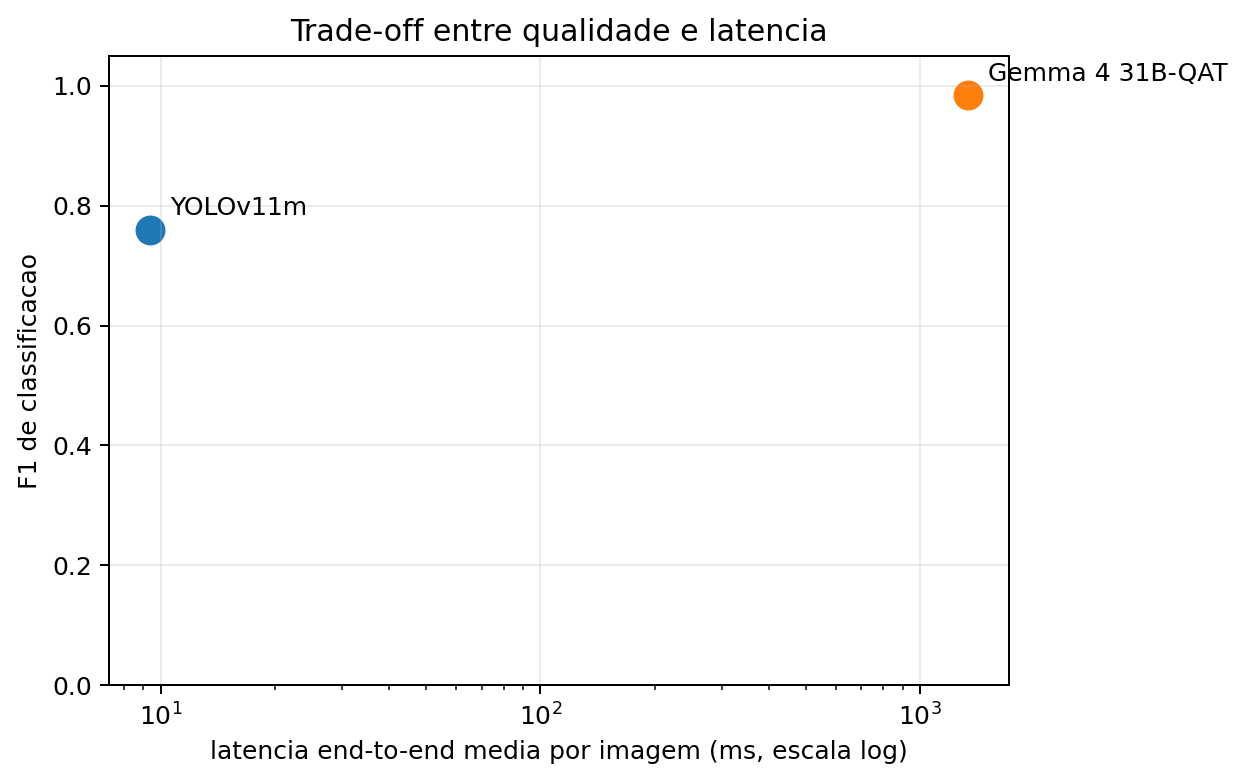
\includegraphics[width=0.72\linewidth]{figures/fig_tradeoff_f1_latencia.png}%
}{%
  \IfFileExists{../outputs/figures/fig_tradeoff_f1_latencia.png}{%
    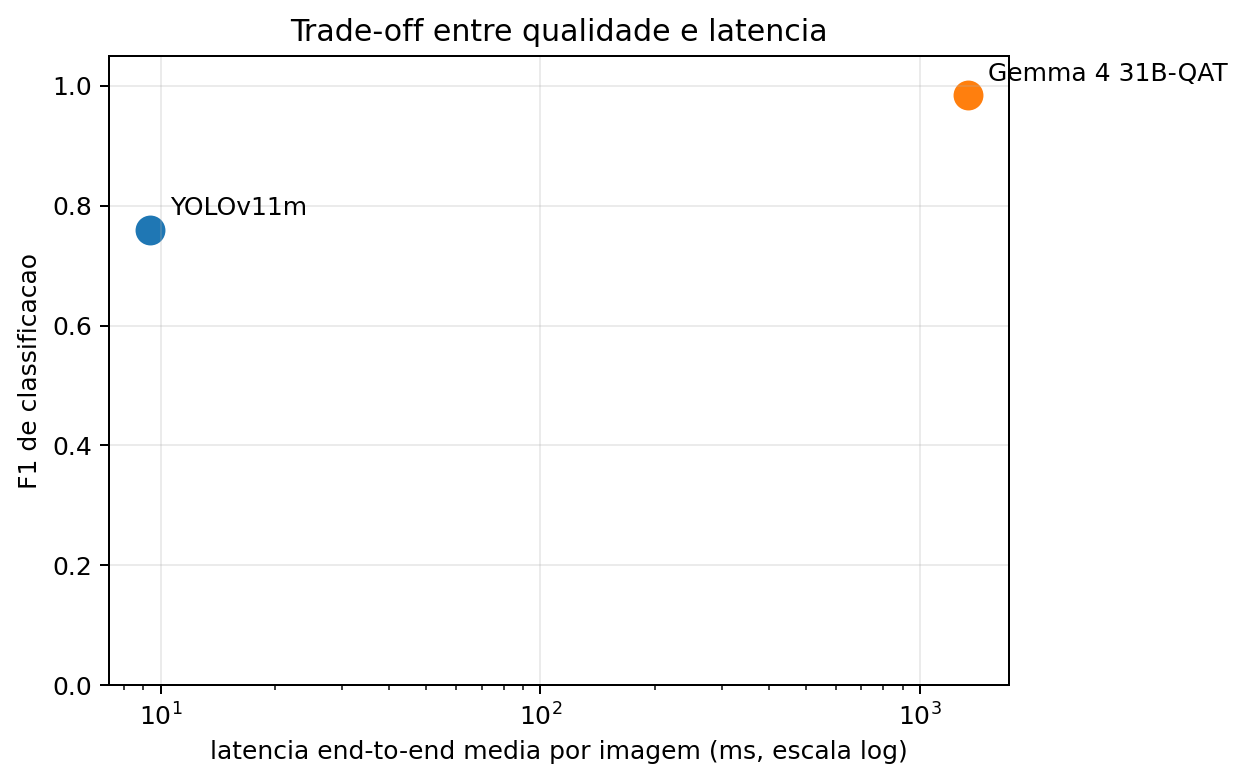
\includegraphics[width=0.72\linewidth]{../outputs/figures/fig_tradeoff_f1_latencia.png}%
  }{%
    \fbox{\parbox{0.68\linewidth}{\centering Figura de trade-off não encontrada. Execute o notebook fonte para gerar o PNG.}}%
  }%
}
\caption{Trade-off entre F1-score e latência média end-to-end. Pontos mais próximos do canto superior esquerdo indicam maior desempenho com menor custo temporal.}
\label{fig:tradeoff-f1-latencia}
\end{figure}

\subsection{Análise dos erros e complementaridade}
\label{sec:analise-erros}

Os modelos acertaram conjuntamente 433 imagens (77,3\% do teste); apenas o Gemma acertou 118, apenas o YOLO acertou 7 e ambos erraram 2. Nos falsos negativos do YOLO foram observados sacos de lixo amassados, molhados, parcialmente oclusos ou pouco contrastados em relação ao pavimento, além de variações de iluminação, perspectiva e enquadramento, sugerindo deslocamento de domínio. O Gemma teve 7 falsos negativos e 2 falsos positivos, indicando maior sensibilidade, mas possível sobre-sinalização contextual. Na localização, os erros se concentraram em caixas desalinhadas, sacos pequenos e múltiplos sacos próximos. A combinação de VLMs com componentes especializados de localização já foi explorada em arquiteturas de detecção e segmentação aberta \cite{Kuo2023FVLM,Lin2024VLSAM}. No contexto deste trabalho, essa evidência motiva avaliar uma cascata em que o detector processa todo o fluxo e o VLM analisa apenas casos selecionados, mas o desempenho dessa arquitetura não é demonstrado pelos experimentos atuais.

\subsection{Implicações para a gestão pública}
\label{sec:implicacoes-gestao}

Os resultados sugerem três usos principais: em monitoramento contínuo, o YOLOv11m é preferível pela baixa latência, alto \emph{throughput} e geração nativa de caixas, desde que recalibrado ao domínio local; em auditorias pontuais, o Gemma 4 31B-QAT é mais indicado quando a qualidade da identificação prevalece; e, em triagens com confirmação, uma arquitetura híbrida pode combinar velocidade e sensibilidade. Em todos os cenários, a adoção deve incluir revisão humana, auditoria de decisões, monitoramento de desempenho e reavaliação periódica.

\section{Ameaças à Validade}
\label{sec:ameacas-validade}

As ameaças à validade externa decorrem principalmente do recorte do conjunto de teste. A avaliação usou uma amostra balanceada artificialmente, com 50\% de imagens positivas, útil para comparação controlada, mas distinta da prevalência esperada em monitoramento contínuo de vias públicas. Embora o teste utilize imagens brasileiras, ele ainda representa um subconjunto específico de cenas, horários, enquadramentos e condições urbanas; assim, os resultados devem ser interpretados como evidência comparativa no domínio avaliado, não como estimativa direta para qualquer cidade, câmera ou política operacional.

Quanto à validade de construto, a tarefa foi reduzida à presença de sacos de lixo visíveis, sem estimar conteúdo, volume ou risco sanitário. A avaliação espacial por IoU 0,5 é diagnóstica, pois o VLM retorna até cinco caixas sem confiança. A anotação primária de cada imagem foi feita por um pesquisador e revisada pelo outro; o consenso reduz divergências, mas não produz uma medida independente de concordância interanotador.

As ameaças à validade interna decorrem da assimetria entre as estratégias: a comparação reflete formas de implantação distintas, e não uma comparação isolada entre arquiteturas. O YOLO foi ajustado com supervisão específica, enquanto o Gemma 4 31B-QAT se beneficia de pré-treinamento multimodal em larga escala. Comparações desse tipo dependem do alinhamento entre os conceitos aprendidos pelo modelo fundacional e as definições adotadas no conjunto-alvo \cite{Madan2024FewShotVLM}; o possível \emph{domain shift} pode afetar especialmente o detector. A validade de conclusão é mitigada por métricas pareadas, intervalos de confiança e teste de McNemar, mas a eficiência representa os fluxos implementados: Gemma via LM Studio 0.4.15 (Build 2), artefato GGUF Q4\_0 e HTTP, sem experimentos de concorrência, energia ou custo em produção.

\section{Conclusão}
\label{sec:conclusao}

Este trabalho comparou YOLOv11m e Gemma 4 31B-QAT na identificação e localização de sacos de lixo em 560 imagens de vias públicas brasileiras. O Gemma obteve melhor desempenho binário e melhor localização aproximada, mas os baixos F1-scores por caixas mostram que a localização fina permanece aberta. O YOLO foi substancialmente mais rápido e forneceu caixas nativas para validação visual.

Os resultados não sustentam a adoção universal de um único modelo: o Gemma favorece análises orientadas à qualidade preditiva, enquanto o YOLO é mais apropriado a triagens em larga escala. Trabalhos futuros devem ampliar a base municipal, refinar a avaliação espacial, testar modelos menores, quantificar custos energéticos e avaliar sistemas híbridos de triagem e confirmação.

\noindent\textbf{Disponibilidade de código e dados.} Os artefatos de reprodução e o notebook estão disponíveis em \url{https://github.com/jaimejrs/urban-waste-yolo-vs-vlm}. A publicação das imagens observará as licenças, os termos do Google Street View e os procedimentos de anonimização.

\bibliographystyle{kdmile}
\bibliography{urban-waste-yolo-vs-vlm}

\begin{received}
\end{received}

\end{document}
